\documentclass[fsharpNotes.tex]{subfiles}
\graphicspath{ {./figures/} }

\begin{document}

\chapter{Organising Code in Libraries and Application Programs}
\label{chap:modules}

\abstract{
  We have previously seen how code can be organized into functions to make programs easier to read, make code pieces reusable, and make programs easier to debug. Functions and values may further be grouped into libraries, and the \lstinline{List} module is an example of such a library that you have already used. F\# includes several programming structures to organize code in libraries: Modules, namespaces, and classes. In this chapter, we will focus on modules. Classes will be described in detail in \Cref{chap:oop}. Here you  will learn how to:
  \begin{itemize}
  \item Use the \lstinline[language=console]{dotnet} command-line tool to create project files and how to compile these into an executable file.
  \item The difference between running interpreted and compiled programs.
  \item Make libraries using modules and write applications using such libraries.
  \item Specify the abstract structure of a module using signature files.
  \item Create an implementation of the Stack abstract datatype.
  \item Update an integer stack to a generic stack.
  \end{itemize}
}


\section{Dotnet projects: Libraries and applications}
\label{chap:projects}
As our programs grow in size, it can be convenient to split the program over several files, e.g., by separating functionality into something general and specific for the problem being solved. An example of this is the \lstinline{List} module which contains general functions on lists, and which you have used in your programs. In this chapter, we will write modules ourselves, also known as libraries, and the programs using these libraries, we will call applications. Using the \lstinline[language=console]{dotnet} command-line tool, we are able to create project files which have a \lstinline[language=console]{.fsproj} suffix, which include information about which source code and packages belongs together. The \lstinline[language=console]{dotnet} command-line tool can help structure the files on the filesystem by use of directories, but here we advocate for a simple, hand-held solution.

To make a light version of \lstinline[language=console]{dotnet} project with a library and an application file, start by creating the \lstinline[language=console]{dotnet} project template as follows:
\begin{codeNOutput}[label=dotnetNew,
  top=-5pt,
  bottom=-5pt,
  left=-2pt,
  right=-2pt,
]{: Creating an initial library-application file setup.}
  \begin{lstlisting}[language=console,escapechar=§]
$ dotnet new console -lang "F#" -o app
\end{lstlisting}%$
\end{codeNOutput}
This creates the \lstinline[language=console]{app} directory with among other things a \lstinline[language=console]{Program.fs} file. The \lstinline[language=console]{Program.fs} is the default filenames for an application. Usually, the \lstinline[language=console]{.fs} suffix is reserved for libraries, so, rename \lstinline[language=console]{Program.fs} to \lstinline[language=console]{Program.fsx}. Then create a possibly empty library file \lstinline[language=console]{Library.fs} using a standard editor. You should now have a directory as shown in \Cref{fig:dotnetNewLightFileSystem}.
\begin{figure} % make sure figure is printed after the countRecursive
  \centering
  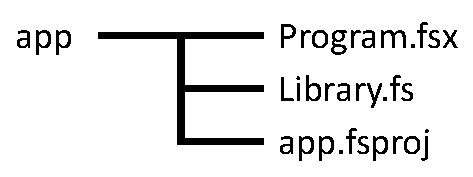
\includegraphics[width=0.35\linewidth]{dotnetLightNew}
  \caption{A set of files for a light version of a dotnet project.}
  \label{fig:dotnetNewLightFileSystem}
\end{figure}
 The \lstinline[language=console]{.fsproj} file is an XML-file which describes how dotnet should combine various files. The \lstinline[language=console]{dotnet} command-line tool can edit this file, but we might as well do this ourselves in a text editor: Open the file in your favorite text editor and in the \lstinline[language=console]{<ItemGroup>} change \lstinline[language=console]{Program.fs} to \lstinline[language=console]{Program.fsx} and add a line with the name of your library file \lstinline[language=console]{<Compile Include="Library.fs" />}. The resulting file should look like this:
\begin{codeNOutput}[label=appLightFsproj,
  top=-5pt,
  bottom=-5pt,
  left=-2pt,
  right=-2pt,
]{: The initial content of \texttt{app.fsproj}.}
  \begin{lstlisting}[language=console,escapechar=§]
<Project Sdk="Microsoft.NET.Sdk">
 <PropertyGroup>
  <OutputType>Exe</OutputType>
  <TargetFramework>net6.0</TargetFramework>
 </PropertyGroup>
 <ItemGroup>
  <Compile Include="Library.fs" />
  <Compile Include="Program.fsx" />
 </ItemGroup>
</Project>
\end{lstlisting}
\end{codeNOutput}
If you decide to rename the application or library files, then you must update the project files accordingly.

If you wish to add references to packages such as the \lstinline{DIKU.Canvas} package, this can be done as,
\begin{codeNOutput}[label=dotnetAdd,
  top=-5pt,
  bottom=-5pt,
  left=-2pt,
  right=-2pt,
]{: Creating an initial library-application file setup.}
  \begin{lstlisting}[language=console,escapechar=§]
$ dotnet add app/app.fsproj package "DIKU.Canvas" --version 1.0.1
\end{lstlisting}%$
\end{codeNOutput}
or manually by editing the project file appropriately. When a package is included in the project file, then it does not need to be loaded in libraries and applications using the \lstinline{#r} directive. This version will compile and run the library and the program, but will not build the library separately.

The order of the references to packages, libraries, and application files are important, since \lstinline[language=console]{dotnet} will read them from top to bottom, and only if, e.g., \lstinline[language=console]{Library.fs} is above \lstinline[language=console]{Program.fsx} will the library functions be available in the application.

As an example, change \lstinline[language=console]{Program.fs} to become what is shown in \Cref{program},
\fsImplementation{solution/app/Program}{program}{A simple application program.}{}
change \lstinline[language=console]{Library.fs} to become what is shown in \Cref{library}, 
\fsImplementation{solution/library/Library}{library}{A simple library.}{}
and run it in \idx{compile mode} by changing to the \lstinline[language=console]{app} directory and using the \lstinline[language=console]{dotnet run} command as demonstrated in \Cref{dotnetRun}.
\begin{codeNOutput}[label=dotnetRun,
  top=-5pt,
  bottom=-5pt,
  left=-2pt,
  right=-2pt,
]{: Running an application setup with one or more project files.}
  \begin{lstlisting}[language=console,escapechar=§]
$ cd solution/app
$ dotnet run
"Greetings Jon"
\end{lstlisting}%$
\end{codeNOutput}
Assuming that \lstinline[language=console]{Program.fs} was renamed to \lstinline[language=console]{Program.fsx} and \lstinline[language=console]{app.fsproj} was edited appropriately, \lstinline[language=console]{dotnet run} is almost the same as
\begin{codeNOutput}[label=dotnetFsi,
  top=-5pt,
  bottom=-5pt,
  left=-2pt,
  right=-2pt,
]{: Running an application setup with one or more project files.}
  \begin{lstlisting}[language=console,escapechar=§]
$ dotnet fsi ../library/Library.fs Program.fsx
"Greetings Jon"
\end{lstlisting}%$
\end{codeNOutput}
However, \lstinline[language=console]{dotnet fsi} \idx{interprets} the library and application into executable code everytime it is called, while \lstinline[language=console]{dotnet run} only \idx{compiles} the program once. On my laptop, the time these different steps take depends on what else is running on the computer, but typical timings are
\begin{center}
  \rowcolors{2}{oddRowColor}{evenRowColor}
  \begin{tabular}{|l|l|}
    \hline
    \rowcolor{headerRowColor} Command & Time\\
    \hline
    \lstinline[language=console]|dotnet fsi ../library/Library.fs Program.fsx| & 1.2s\\
    \lstinline[language=console]|dotnet run| (first time) & 4.0s\\
    \lstinline[language=console]|dotnet run| & 1.0s\\
    \hline
\end{tabular}
\end{center}
The example application, we are studying here, is tiny, but even in this case, the repeated translation by \lstinline[language=console]{dotnet fsi} is a 16\% overhead when compared to an already compiled program, and you should expect this overhead to be larger for larger programs. However, for tiny programs, the cost of the initial compilation is 400\% and not worth the effort from a time perspective.


\section{Libraries and applications}
\label{sec:modules}
A library in F\# is expressed as a \idx{module}, which is a programming structure used to organize type declarations, values, functions, etc. The libraries should have the suffix \lstinline[language=console]{.fs}, and here will call them \idx{implementation files} in contrast to the signature files to be discussed below, which we will call \idx{signature files}.

A module is typically a file where the module name is declared in the first lines using the \idx[module@\lstinline{module}]{\keyword{module}} with the following syntax,
%
\begin{verbatimwrite}{\ebnf/outerModule.ebnf}
module <*ident*>
<*script*>
\end{verbatimwrite}
\syntax{\ebnf/outerModule.ebnf}{Outer module.}
%
Here, the identifier \lstinline[language=syntax]{<*ident*>} is a name not necessarily related to the filename, and the script \lstinline[language=syntax]{<*script*>} is an expression.

Consider the example from \Cref{solveQuadraticEquation} in which functions are defined for solving the values of $x$ where $f(x)=0$ for a quadratic equation. In the following, we will split this into a library of functions and an application program. For this, we set up a project system of files as described in \Cref{chap:projects}, where \lstinline[language=console]{Program.fs} has been replaced by \lstinline[language=console]{Program.fsx} and the \lstinline[language=console]{app.fsproj} has been edited appropriately. The content of  \lstinline[language=console]{Library.fs} has been changed to become what is shown in \Cref{quadraticModule}, 
\fsImplementation{solve/library/Library}{quadraticModule}{A library for solving quadratic equations.}{}
and \lstinline[language=console]{Program.fsx} has been changed to what is shown in \Cref{quadraticApp}.
\fsCode{solve/app/Program}{quadraticApp}{An application using the \lstinline!Solve! module.}{}

\section{Specifying a Module's Interface with a Signature File}
As the 8-step guide suggests, the design of programs is helped by first considering what the program's function is to do before actually implementing them. This also holds for libraries, and signature files can aid this process. 

A \idx[signature file]{signature files} is a file accompanying \idx{implementation files} and have the suffix \lstinline[language=console]{.fsi}. A signature file contains almost no implementation, but only type definitions. Signature files offer three distinct features:
\begin{enumerate}
\item Signature files can be used as part of the documentation of code since type information is of paramount importance for an application programmer to use a library. 
\item Signature files may be written before the implementation file. This allows for a higher-level programming design that focuses on \emph{which} functions should be included and \emph{how} they can be composed.
\item Signature files allow for access control. Most importantly, if a type definition is not available in the signature file, then it is not available to the application program. Such definitions are private and can only be used internally in the library code. More fine-grained control related to classes is available and will be discussed in \Cref{chap:oop}.
\end{enumerate}
These features help the programmer structure the process of programming and protect the user of a library from irrelevant data and functions. A signature file contains the type definitions and the types of values and functions to be exposed to the user of the library. For example, for the library in \Cref{quadraticModule}, we can define a signature files which makes the \lstinline{solveQuadraticEquation} function but not the \lstinline{discriminant} function available to the user of the library as demonstrated in \Cref{librarySignature}.
\fsSignature{solve/library/Library}{librarySignature}{A signature file for \Cref{quadraticModule}.}{}
To compile the application using the signature file, we must add the created file, e.g., \lstinline[language=console]{Library.fsi}, to the project file as, e.g., shown in \Cref{libraryFsprojFSI}.
\begin{codeNOutput}[label=libraryFsprojFSI,
  top=-5pt,
  bottom=-5pt,
  left=-2pt,
  right=-2pt,
]{: The \texttt{library.fsproj} with a signature file added.}
  \begin{lstlisting}[language=console,escapechar=§]
<Project Sdk="Microsoft.NET.Sdk">
 <PropertyGroup>
  <OutputType>Exe</OutputType>
  <TargetFramework>net6.0</TargetFramework>
 </PropertyGroup>
 <ItemGroup>
  <PackageReference Include="DIKU.Canvas" Version="1.0.1" />
  <Compile Include="Library.fsi" />
  <Compile Include="Library.fs" />
  <Compile Include="Program.fsx" />
 </ItemGroup>
</Project>
\end{lstlisting}
\end{codeNOutput}
In the context of the 8-step guide, it is useful to write the signature file before the implementation file, and that the signature file contains the documentation for the functions available in the application.

For technical reasons in the  \lstinline[language=console]{dotnet} framework, exposed type abbreviations must be given both in the signature file and the implementation file. The implication is that the signature at times must also define implementation details, see e.g., the example below, and thus becomes less abstract the desirable in general.

\section{Programming Intermezzo: Postfix Arithmetic with a Stack}
\label{sec:stack}
To this point, we have performed simple arithmetic using \idx{infix} notation, meaning that expressions like $(4+6*3)/2-8$ are evaluated using the precedence and association rules of the operators as
\begin{align}
  (4+6*3)/2-8
  &\rightsquigarrow (4+18)/2-8\\
  &\rightsquigarrow 22/2-8\\
  &\rightsquigarrow 11-8\\
  &\rightsquigarrow 3
\end{align}
However, there is an equally valid notation, \idx{postfix}, in which the same expression is written as $4\; 6\; 3\; *\; +\; 2\; /\; 8\; -$. Here, the rule is to read from left to right, and whenever there are two values and an operator, $a\; b\; \text{op}$, replaced this with the value $a \text{ op } b$ and repeat until only one value remains, which is the result of the calculation. Hence,
\begin{align}
  4\; 6\; 3\; *\; +\; 2\; /\; 8\; -
  &\rightsquigarrow\; 4\; 18\; +\; 2\; /\; 8\; -\\
  &\rightsquigarrow\; 22\; 2\; /\; 8\; -\\
  &\rightsquigarrow\; 11\; 8\; -\\
  &\rightsquigarrow\; 3
\end{align}
This was implemented on a series of calculators released by Hewlett-Packard in the 1960-1980'ies, and one of the arguments for this notation was, that the expressions could be evaluated by a stack with only 3 levels. In the following, we will look at stacks as an abstract datatype and build a library for stacks and an arithmetic solver for such simple expressions using this stack.

A stack is an abstract datatype, meaning that it is defined by its concepts, not its implementation. The concept of a stack is like a stack of plates in a cafeteria, they are placed in a physical stack, and you can take the top plate and place a plate on the top, but you cannot access a plate in the middle of a stack. Stacks typically come with the following functions:
\begin{description}
\item[create:] Create an empty stack.
\item[pop:] Return the top element and the resulting stack.
\item[push:] Put an element on a stack and return the resulting stack.
\item[isEmpty:] Check whether the stack is empty.
\end{description}
Following the 8-step guide \Cref{sec:8step}, the above directly suggests names and includes brief descriptions (Steps 1 and 2). Step 3 suggests that we write a simple test, and
since we are fond of piping, our test program is shown in \Cref{postfixTestCode}.
\fsCode{postfixTest}{postfixTestCode}{A simple program using a yet to be written library.}{}
We expect this to print the result of the last \lstinline{pop} call, which should include information about the element \lstinline{2}.

In the functional programming paradigm, our stack is a constant, implying that every time we pop and push, we create new stacks. Thus, for step 4 in the 8-step guide, we must accept that all but \lstinline{isEmpty} returns a new stack, and all but \lstinline{create} must take a stack as input. Thus we arrive at a signature file for the stack-library given in \Cref{postfixLibrarySignature}.
\fsSignature{postfixLibrary}{postfixLibrarySignature}{A signature file for the stack library}{} 
A limitation to F\#'s modules is that the type specifications need explicit declaration. We would have liked to write \lstinline{type stack} and functions of some variable type \lstinline{'e}, since the stack concept is independent of the type of elements it contains. However, this is not possible, and thus, we here specialize to float stacks. For similar reasons, we are forced to specify details about the implementation of our type. Our idea is that stacks can be implemented as lists since lists are well suited to work with the first elements.

Implementing a stack using lists is simple, since lists already contains the properties \lstinline{Head}, \lstinline{Tail}, and \lstinline{IsEmpty}, which closely mimics the needed operations for a stack. Thus we arrive at \Cref{postfixImplementation}.
\fsImplementation{postfixLibrary}{postfixImplementation}{An implementation of a stack module.}{}
And now we can run our test code as shown in \Cref{postfixTest}.
\fsOutput{postfixTest}{Running the test program}
As expected, the top element and the resulting stack is \lstinline{(2,[1])}.

To implement simple postfix algebra, we will use discriminated unions. That is, we define a type,
\begin{quote}
\lstinline{type element = Value of int | Multiply | Plus | Minus | Divide}
\end{quote}
This allows us to make lists of tokens such as,
\begin{quote}
\lstinline{[Value 4; Value 6; Value 3; Multiply; Plus]}
\end{quote}
for the expression $3\; 4\; 2\; /\; +$ which is equivalent to $3+4/2$ in infix notation. The next step is to understand how to use a stack to evaluate such expressions. The idea is to process the list of tokens from its head and push values to a stack. When the head of the tokens list is an operator, say 'op' then the two top elements from the stack are popped, say $a$ and $b$, the mathematical expression $c = a\text{ op }b$ is evaluated and $c$ is pushed to the stack. For our example, the evolution of the stack will be:
\begin{center}
  \begin{tabular}{l|r}
  Unused tokens &  Evaluation stack\\\hline
  $4\; 6\; 3\; *\; +\; 2\; /\; 8\; -$ & \lstinline![]! \\
  $6\; 3\; *\; +\; 2\; /\; 8\; -$ & \lstinline![4]! \\
  $3\; *\; +\; 2\; /\; 8\; -$ & \lstinline![6; 4]! \\
  $*\; +\; 2\; /\; 8\; -$ & \lstinline![3; 6; 4]! \\
  $+\; 2\; /\; 8\; -$ & \lstinline![18; 4]! \\
  $2\; /\; 8\; -$ & \lstinline![22]! \\
  $/\; 8\; -$ & \lstinline![2; 22]! \\
  $8\; -$ & \lstinline![11]! \\
  $-$ & \lstinline![8; 11]! \\
   & \lstinline![3]! \\
\end{tabular}
\end{center}
As demonstrated, the result of the expression is the last element on the stack, once the list of tokens is empty. An F\# implementaiton is given in \Cref{postfixApp}.
\fs{postfixApp}{An application for evaluating lists of tokens on postfix form using a stack.}

\section{Generic Modules}
\label{sec:genericModule}
The stack is an example of an abstract datatype, and in the previous section, we implemented a stack for floats, however, stacks can be of many other types, and although we could make a stack module for each type, it would greatly improve the usefulness of our library, if we could make a stack module, which is generic, i.e., where the user can decide when writing applications, which type of values to stack. Luckily, this is supported in F\#.

In \Cref{sec:variableTypes} we discussed the usefulness of the variable type such as \lstinline{'a}, which makes functions and types generic, that is, the same definition can be used for any type. To make a generic module, it is often useful first to make a non-generic version, such as our float stack, since it is often easier to spot errors in concrete program versions. The float stack already works as desired, so we will now modify the module to be a stack for a variable type. In our example, we must update both the type abbreviation and function types in the signature file. The result is shown in \Cref{postfixLibraryGenericSignature}.
\fsSignature{postfixLibraryGeneric}{postfixLibraryGenericSignature}{A signature file for the generic stack library}{} 
The next step is to update the implementation file. During such transformations, it is not uncommon to realize that restrictions must be put on the type, which is possible but which we will not consider further in this book. Since the stack does not rely on any properties of the stack elements, there is no challenge in modifying the implementation file as shown in \Cref{postfixLibraryGenericImplementation}.
\fsImplementation{postfixLibraryGeneric}{postfixLibraryGenericImplementation}{An implementation of a generic stack module.}{}
Finally, we can make an application using stacks of various kinds, as shown in \Cref{postfixTestGeneric}.
\fs{postfixTestGeneric}{Running the test program}{}
In the program, we see that F\# can infer that a stack, on which floats are pushed, must be of \lstinline{stack<float>} type, and when characters are pushed, then the stack must be of type \lstinline{stack<char>}. Thus, we have arrived at a stack for any type, whose interface is given by the signature file, and almost all of its implementation is hidden in the implementation file.

\section{Key Concepts and Terms in This Chapter}
In this chapter, we have looked at how to build libraries and applications. Key concepts have been
\begin{itemize}
\item How to build organise the compilation of libraries and applications using \lstinline[language=console]{dotnet} \textbf{project files}.
\item How to design libraries using \textbf{modules} and \textbf{signature files}.
\item How to make \textbf{library implementation files}.
\item How to implement the \textbf{abstract datatype Stack} both as a float stack and as a \textbf{generic module}. 
\end{itemize}

\end{document}

